% @Author: AnthonyKenny98
% @Date:   2020-02-22 15:42:12
% @Last Modified by:   AnthonyKenny98
% @Last Modified time: 2020-04-06 15:04:06

The first objective of this thesis is to identify a typical motion planning algorithm, profile its execution, and determine computational bottlenecks.\todo{Update once I have properly defined goals and objectives}

This chapter introduces the concept of motion planning and details the process of implementing and analyzing \glsfirst{RRT}, a commonly used algorithm, to identify its computational bottlenecks.\\

\section{Motion Planning Background} 
\label{section:motion_planning_background}
    % @Author: AnthonyKenny98
% @Date:   2020-04-04 10:01:40
% @Last Modified by:   AnthonyKenny98
% @Last Modified time: 2020-04-05 10:56:20

A funny paradox in computer science is the fact that it is relatively easy to teach a computer to perform tasks that humans find very complicated, but extremely difficult to program one to execute functions that humans master during infancy. Consider, it was as early as 1949 that Claude Shannon presented his paper \textit{Programming a Computer for Playing Chess}\cite{Shannon1950}, and by 1997 the \textit{Deep Blue} computer defeated Garry Kasparov, reigning world champion, in a six game chess match.\cite{Campbell2002} Compare that with some of the most advanced autonomous humanoid robots to date displaying dexterity only comparable with that of a toddler. The task of finding a collision free path, performed constantly without thought by a human, is an example of this paradigm. For a robot to compute a collision free path, it relies on a set of Motion Planning Algorithms.

Motion Planning Algorithms refer to the set of algorithms that find possible sequences of valid \gls{configuration}s for a robot in a space. In plain English, they are algorithms that determine the movements a robot can make in a map, with the intent of eventually finding a path from one point to another. 

\subsection{Key Concepts}
    \subsubsection{\Gls{workspace}}
    The \gls{workspace}, more loosely known as the \textbf{map}, is the space which the robot and obstacles occupy. Obviously, \textbf{obstacles} refer to anything with which the robot cannot intersect.
    
    \subsubsection{Configuration}
    A configuration describes the position, orientation, and pose of the robot. The complexity of a robot's configuration is therefore dependant on the dimension of the \gls{workspace}, the complexity of the robot itself, and in what level of detail the robot must be represented. For example:
    \begin{itemize}
        \item Most simply, a robot can be represented as a point by the Cartesian coordinates $(x,y)$ \gls{2D} space and $(x,y,z)$ in \gls{3D} space.
        \item More realistically, a robot such as a drone may be represented in \gls{3D} by an origin point $(x,y,z)$ and 3 Euler angles $(\alpha,\beta,\gamma)$ describing its orientation.
        \item In a more complex form, a fixed base robot with $N$ \glsfirst{DOF} would require an $N$-dimensional configuration.
    \end{itemize}

    % @Author: AnthonyKenny98
% @Date:   2020-04-04 11:13:58
% @Last Modified by:   AnthonyKenny98
% @Last Modified time: 2020-04-04 12:09:59
% @Author: AnthonyKenny98
% @Date:   2020-02-29 17:30:44
% @Last Modified by:   AnthonyKenny98
% @Last Modified time: 2020-04-03 14:28:30
\begin{figure}[H]
\begin{center}
\begin{tabular}{cc}

    % Subfigure A
    \begin{subfigure}{0.4\textwidth}
    \begin{center}
    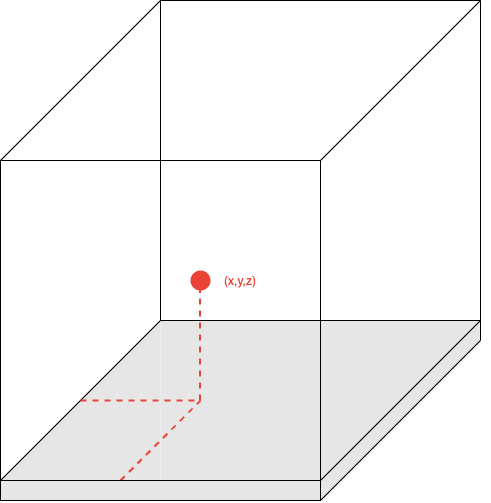
\includegraphics[width=\linewidth]{chapters/chapter2/img/motionPlanning/3DPointConfiguration.png}
    \caption{A robot represented by just a point in 3D space, requiring only 3 Cartesian coordinate $(x,y,z)$ points to describe its \gls{configuration}}
    \label{subfig:3DPointConfig}
    \end{center}
    \end{subfigure}
    &
    % 
    % Subfigure B
    \begin{subfigure}{0.4\textwidth}
    \begin{center}
    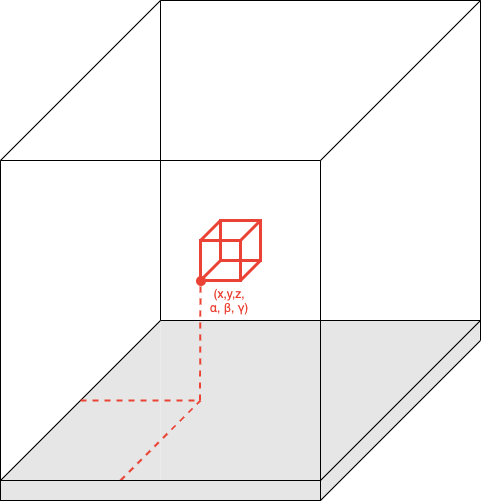
\includegraphics[width=\linewidth]{chapters/chapter2/img/motionPlanning/3DCubeConfiguration.png}
    \caption{A robot represented as a cube in 3D space, now requiring 3 Euler angles $(\alpha, \beta, \gamma)$ along with the original Cartesian coordinates.}
    \label{subfig:3DCubeConfig}
    \end{center}
    \end{subfigure} \\
\end{tabular}
    % Caption and Label
    \caption{Example of 2 Robot Configurations in 3D Space for Motion Planning Purposes}
    \label{fig:configuration}

\end{center}
\end{figure}

    \subsubsection{Occupancy Grid Map}
    An \glsfirst{OGM} is a method of representing the obstacles present in a \gls{workspace}. Obstacles are often irregularly shaped and computing collisions with such obstacles is near impossible. Therefore, the \gls{workspace} is discretized into grids and grids containing any part of the obstacle are markes as occupied, even if only a small part of the grid is occupied. An \gls{OGM} will more accurately represent a \gls{workspace} with a higher resolution, shown in Figure \ref{fig:OGM}.

    % @Author: AnthonyKenny98
% @Date:   2020-04-04 12:27:50
% @Last Modified by:   AnthonyKenny98
% @Last Modified time: 2020-04-06 15:13:14
% @Author: AnthonyKenny98
% @Date:   2020-04-04 11:13:58
% @Last Modified by:   AnthonyKenny98
% @Last Modified time: 2020-04-04 12:09:59
% @Author: AnthonyKenny98
% @Date:   2020-02-29 17:30:44
% @Last Modified by:   AnthonyKenny98
% @Last Modified time: 2020-04-03 14:28:30
\begin{figure}[H]
\begin{center}
\begin{tabular}{cc}

    % Subfigure A
    \begin{subfigure}{0.4\textwidth}
    \begin{center}
    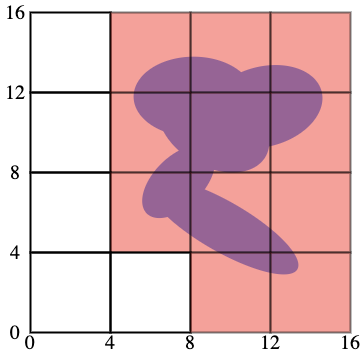
\includegraphics[width=\linewidth]{chapters/chapter2/img/motionPlanning/OGMlowres.png}
    \caption{}
    \label{subfig:OGM_A}
    \end{center}
    \end{subfigure}
    &
    % 
    % Subfigure B
    \begin{subfigure}{0.4\textwidth}
    \begin{center}
    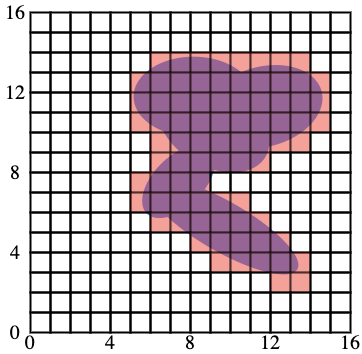
\includegraphics[width=\linewidth]{chapters/chapter2/img/motionPlanning/OGMhighres.png}
    \caption{}
    \label{subfig:OGM_B}
    \end{center}
    \end{subfigure} \\
\end{tabular}
    % Caption and Label
    \mycaption{Occupancy Grid Maps for a (16$\times$16) Workspace of Different Resolutions}{. Figure \ref{subfig:OGM_A} shows how an OGM with low resolution, while simpler to construct and analyse, will over-represent the obstacle density of a workspace. Figure \ref{subfig:OGM_B} shows how a higher resolution will more accurately reflect the obstacles of a workspace.}
    \label{fig:OGM}

\end{center}
\end{figure}

\subsection{Algorithms}
    
    \subsubsection{Scope}
    \todo[inline,caption=Finish Scope]{Part of the problem, it is not about sensing obstacles, building map, or finding shortest path. It is merely about exploring the space and building a tree of possible paths}

\todo[inline]{Finish this Section, should describe why I chose RRT}


\newpage
\section{Implementation of RRT}
\label{section:rrt}
    % @Author: AnthonyKenny98
% @Date:   2020-02-22 15:53:59
% @Last Modified by:   AnthonyKenny98
% @Last Modified time: 2020-04-05 13:31:53

% INTRO
\glsfirst{RRT} is an algorithm designed to efficiently build a tree of collision-free paths in a high-complexity environment. The algorithm randomly samples points, draws an edge from the nearest currently existing node in the tree, to grow the tree in the space. It is inherently biased to grow towards large unsearched areas of the workspace. RRT was developed by S. LaVelle\cite{LaValle1998} and J. Kuffner\cite{LaValle2001}. It is used in autonomous robotic motion planning problems such as autonomous drones.

% ALGORITHM
\subsection{Algorithm}

    % SCOPE OF ALGORITHM
    \subsubsection{Scope}
        \gls{RRT} takes an \glsfirst{OGM} as its input. This \gls{OGM} may be built and updated using \gls{a priori} knowledge, sensor data from the robot, and other inputs. \gls{RRT} will output a tree of collision free paths toward the goal, as demonstrated in Figure \ref{fig:rrt_scope}. \textbf{It does not calculate the fastest path from that tree}; that can be accomplished using algorithms such as \Gls{dijkstra's algorithm}.

        % @Author: AnthonyKenny98
% @Date:   2020-04-05 10:54:20
% @Last Modified by:   AnthonyKenny98
% @Last Modified time: 2020-04-05 11:05:47

\begin{figure}[H]
\begin{centering}
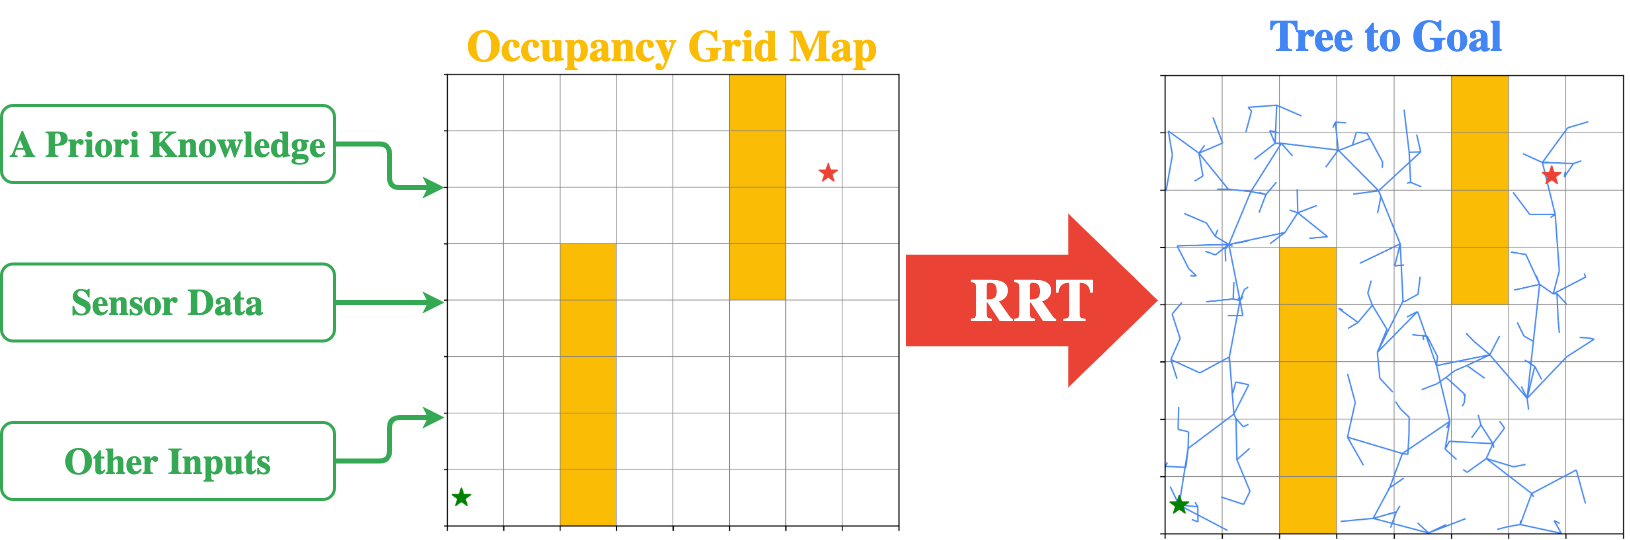
\includegraphics[width=\linewidth]{chapters/chapter2/img/RRT-Scope.png}
\caption[Scope of the RRT Algorithm]{Scope of the RRT Algorithm: Takes an \gls{OGM} as input and outputs a tree of collision free paths through that \gls{OGM}. The tree is shown in blue on the right.} 
\label{fig:rrt_scope}
\end{centering}
\end{figure}

    % BASIC RRT - BUILDING THE TREE
    \subsubsection{Building the Tree}

        Put simply, \gls{RRT} finds a path from start to finish by randomly exploring a workspace.
        Put more technically, it builds a tree of possible \glspl{configuration} (also known as a graph), connected by edges, for a robot of some physical description. It does so by selecting random \glspl{configuration} and adding them to the graph. 
        From this graph, a path from the initial \gls{configuration} to some goal \gls{configuration} can be found, given a high enough number of iterations. As such, \gls{RRT} can be considered \gls{probabilistically complete}.
        The pseudo-code for \gls{RRT} can be seen in Algorithm \ref{algorithm:rrt}
        
        % RRT Algorithm
        % @Author: AnthonyKenny98
% @Date:   2020-02-27 10:55:29
% @Last Modified by:   AnthonyKenny98
% @Last Modified time: 2020-02-27 15:45:23

\begin{algorithm}[H]
    \caption{Rapidly-Exploring Random Tree in Free Configuration Space}
    \SetAlgoLined
    \SetArgSty{textnormal}
    \begin{tabular}{l l}
    \textbf{Inputs:}    & Initial configuration $q_{init}$,\\ 
                        & Number of nodes in graph $K$, \\
                        & Incremental Distance $\Delta q$ \\
    \textbf{Output:}    & RRT Graph $G$ with $K$ configurations \& edges \\
    \end{tabular}

        $G$.init()\;
        \For{$k = 1$ to $K$}{
            $q_{rand} \leftarrow $ randomConfiguration(); \\
            $q_{near} \leftarrow $ nearestVertex($q_{rand}$, $G$); \\
            $q_{new} \leftarrow $ newVertex($q_{near}$, $q_{rand}$, $\Delta q$); \\
            $G$.addVertex($q_{new}$); \\  
            $G$.addEdge($q_{near}$, $q_{new}$);
        }
\label{algorithm:rrt}
\end{algorithm}

        % Explanation of Algorithm, referencing visual step by step figure
        Algorithm \ref{algorithm:rrt} can be visually represented in Figure \ref{fig:rrt-step-by-step}. Consider a \gls{2D} robot operating in a \gls{2D} workspace. A Graph $G$ is initialized containing an initial \gls{configuration}, $q_{init}$, with constraints on the number of nodes that the graph can hold, $K$, and the maximum distance between two nodes, $\Delta q$. This is shown in Sub-figure \ref{subfig:rrt-step-by-step-A}. A random \gls{configuration} for the robot, $q_{rand}$ is generated (\ref{subfig:rrt-step-by-step-B}). The nearest existing \gls{configuration} in $G$, $q_{near}$, is found. (In the first iteration, $q_{near} = q_{init}$, shown in Sub-figure \ref{subfig:rrt-step-by-step-C}). The distance between $q_{near}$ and $q_{rand}$ is calculated. If this distance is less than $\Delta q$, $q_{new} = q_{rand}$. If not, $q_{new}$ is selected, typically by moving by $\Delta q$ from $q_{near}$ towards $q_{rand}$ (\ref{subfig:rrt-step-by-step-C}). $q_{new}$ is then added to $G$. This is repeated for $K$ \gls{configuration}s.
        \todo[inline]{This is all really ugly and should be explained better}

        % Step By Step RRT Figure
        % @Author: AnthonyKenny98
% @Date:   2020-02-27 14:22:10
% @Last Modified by:   AnthonyKenny98
% @Last Modified time: 2020-02-27 15:36:30

\begin{figure}[H]
\begin{center}
\begin{tabular}{c c}

    % Subfigure A
    \begin{subfigure}{0.45\textwidth}
    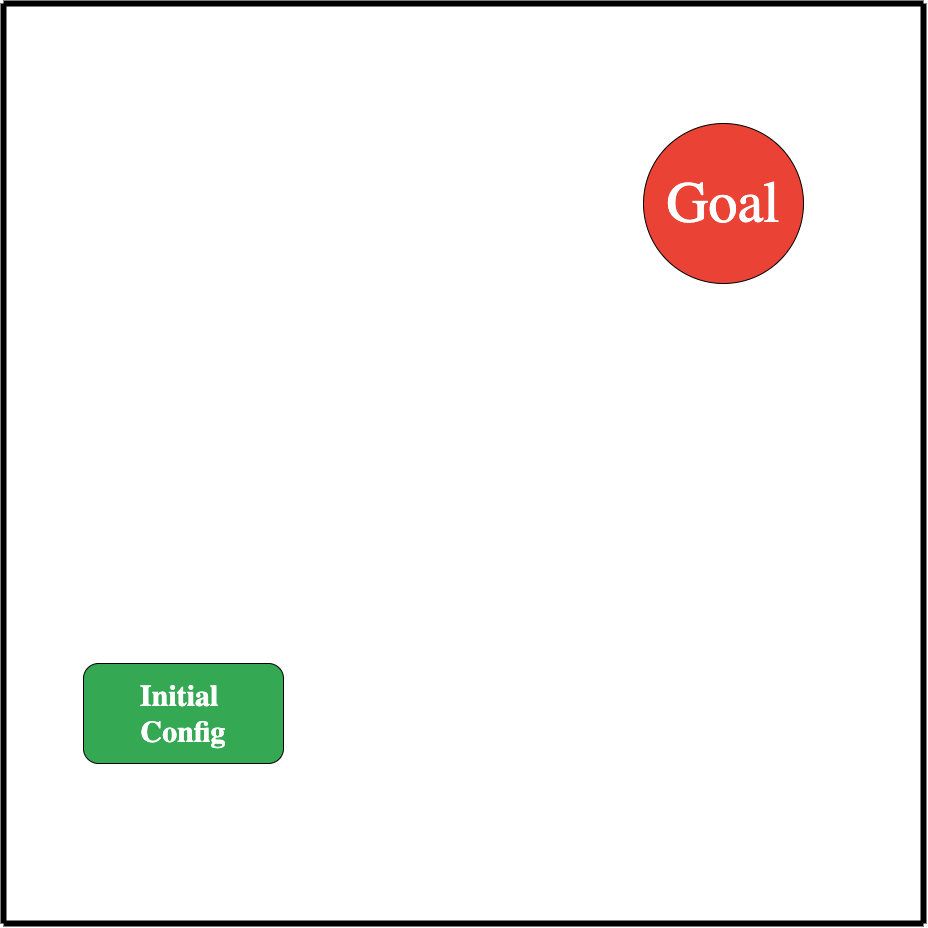
\includegraphics[draft=false,width=\linewidth]{chapters/chapter2/img/RRT_step_by_step-A.png}
    \caption{Graph $G$ contains only $q_{init}$ \newline}
    \label{subfig:rrt-step-by-step-A}
    \end{subfigure} &
    % 
    % Subfigure B
    \begin{subfigure}{0.45\textwidth}
    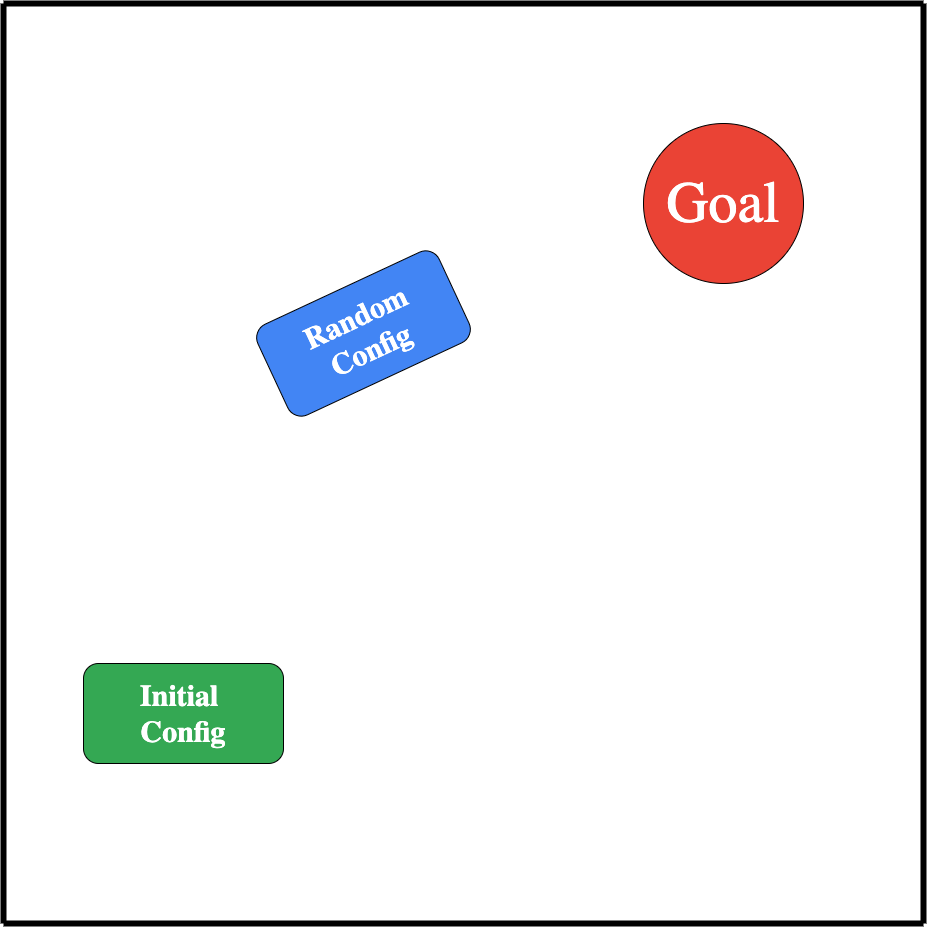
\includegraphics[draft=false,width=\linewidth]{chapters/chapter2/img/RRT_step_by_step-B.png}
    \caption{The first random configuration, $q_{rand}$, is generated}
    \label{subfig:rrt-step-by-step-B}
    \end{subfigure} \\ \\

    % Subfigure C
    \begin{subfigure}{0.45\textwidth}
    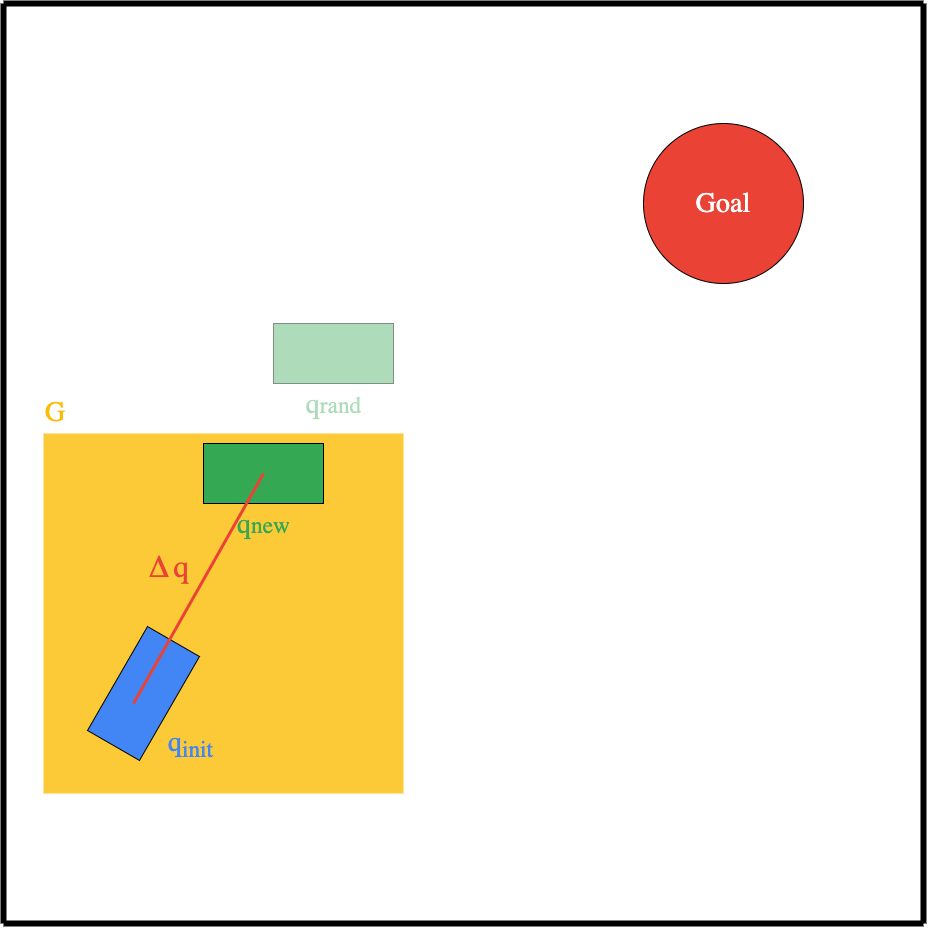
\includegraphics[draft=false,width=\linewidth]{chapters/chapter2/img/RRT_step_by_step-C.png}
    \caption{In first iteration, $q_{near} = q_{init}$. Distance between $q_{init}$ and $q_{rand}$ is greater than $\Delta q$, so $q_{new}$ is generated and added to $G$}
    \label{subfig:rrt-step-by-step-C}
    \end{subfigure} &
    % 
    % Subfigure D
    \begin{subfigure}{0.45\textwidth}
    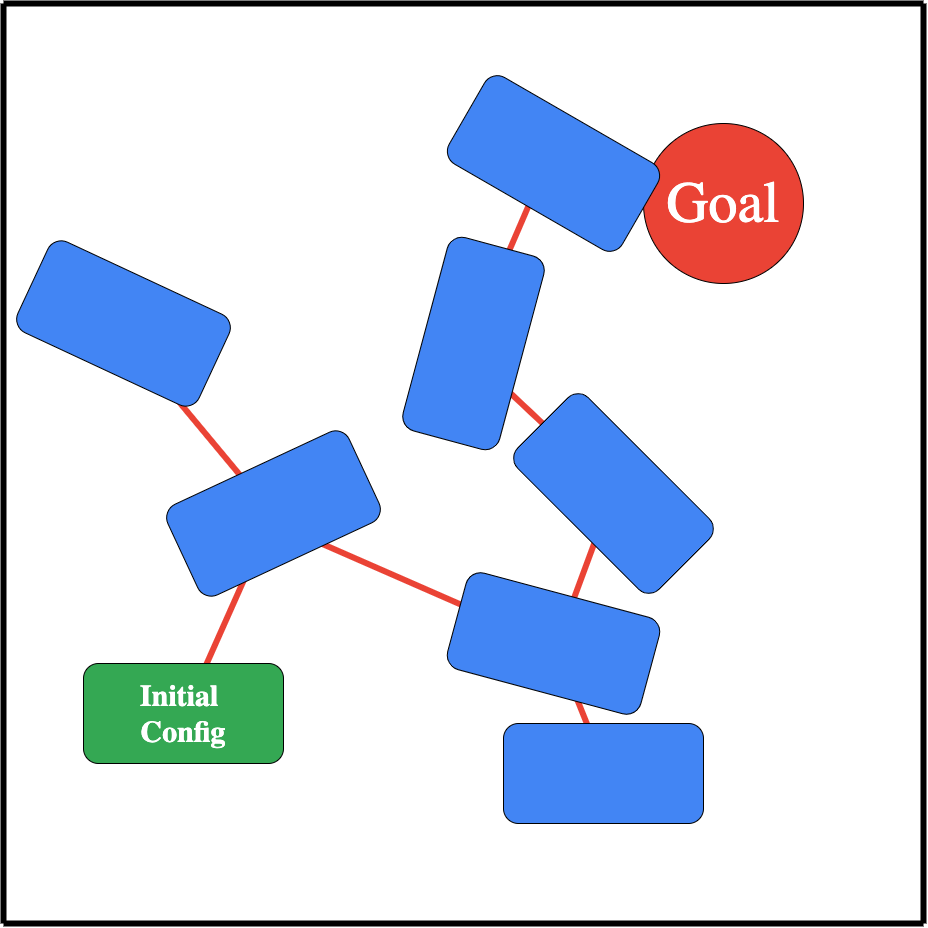
\includegraphics[draft=false,width=\linewidth]{chapters/chapter2/img/RRT_step_by_step-D.png}
    \caption{This is repeated $K$ times. For $G$, $K=10$, and the red line represents the edges between configurations}
    \label{subfig:rrt-step-by-step-D}
    \end{subfigure}

\end{tabular}
    
    % Caption and Label
    \caption{Step by step demonstration of \ac{RRT} Algorithm for 2D robot in 2D space}
    \label{fig:rrt-step-by-step}
\end{center}
\end{figure}
        \todo{Redo this diagram}

    % COLLISION DETECTION
    \subsubsection{Collision Detection}

        Algorithm \ref{algorithm:rrt} shows how \gls{RRT} builds a graph of possible \gls{configuration}s connected by edges in a completely free \gls{configuration} space. However, in real-world applications, a robot's \gls{workspace} space often contains obstacles. As such, collision detection must be included in the algorithm. The two types of collisions the algorithm must check for are \textit{configuration collisions} (those where the robot would collide with an obstacle in a given \gls{configuration}) and \textit{edge collisions} (where the robot would collide when moving between two collision free \gls{configuration}s).

        The RRT with \gls{configuration} and edge collision detection can be seen in Algorithm \ref{algorithm:rrt_collision}. The method of implementing \gls{RRT} with collision detection to model a drone in 3D space is detailed in Section \ref{section:implementation}.

        % @Author: AnthonyKenny98
% @Date:   2020-02-27 18:27:36
% @Last Modified by:   AnthonyKenny98
% @Last Modified time: 2020-04-03 14:28:31
\bigskip
\begin{algorithm}[H]
    \caption{Rapidly-Exploring Random Tree with Collision Detection}
    \SetAlgoLined
    \SetArgSty{textnormal}
    \begin{tabular}{l l}
    \textbf{Inputs:}    & Initial \gls{configuration} $q_{init}$,\\ 
                        & Number of nodes in graph $K$, \\
                        & Incremental Distance $\Delta q$, \\
                        & Space $S$ containing obstacles \\
    \textbf{Output:}    & RRT Graph $G$ with $K$ \gls{configuration}s $[q]$ \& edges $[e]$ \\
    \end{tabular}

        $G$.init()\;
        \For{$k = 1$ to $K$}{
            \While { !\text{pointCollision}($q_{new}$) } {
                $q_{rand} \leftarrow $ randomConfiguration(); \\
                $q_{near} \leftarrow $ nearestVertex($q_{rand}$, $G$); \\
                $q_{new} \leftarrow $ newVertex($q_{near}$, $q_{rand}$, $\Delta q$); \\
            }
            $e_{new} \leftarrow $ newEdge($q_{near}, q_{new}$) \\
            \eIf{\text{!edgeCollision($e_{new}$)}} {
                $G$.addVertex($q_{new}$); \\  
                $G$.addEdge($q_{near}$, $q_{new}$);
            }{
                $k = k-1$;
            }
        }
\label{algorithm:rrt_collision}
\end{algorithm}
\bigskip

\newpage

% IMPLEMENTATION OF RRT
\subsection{Implementation}\label{section:implementation}
    
    % TECHNICAL SPECIFICATIONS
    \subsubsection{Technical Specifications}

        With \gls{RRT} selected as the benchmark algorithm against which to test specialised hardware, this project required an implementation of the algorithm that satisfied the following criteria.\todo{Better RRT Implementation introductory sentence}

        % Tech Spec Table
        \begin{table}[H]
\begin{center}
\begin{tabular}{|p{.3\linewidth}|p{.64\linewidth}|}
    \hline
    Requirement             & Description and Justification \\
    \hline
    C/C++ Implementation    & As outlined in Section \ref{subsection:project_structure}, the critical step in determining the design of specialized hardware to accelerate \ac{RRT} is CPU performance analysis of the algorithm to determine computational hot-spots. Implementations in C allow for the use of certain CPU profiling tools, described in Section \ref{subsubsection:vtune}, unlike higher-level languages such as Python. \\
    \hline
    Models Drone as Point   & In reality, implementing \ac{RRT} for a drone would model the robot as a \ac{3D} object defined by coordinates $\{x, y, z\}$ and Euler angles $\{\alpha, \beta, \gamma \}$. However, for simplicity's sake, modelling the drone as a point defined by coordinates $\{x, y, z\}$ will suffice. Time permitting, this could be revisited. \todo[inline]{Change this based on whether time does permit} \\
    \hline
    Mirrors Algorithm       & In order for the results of CPU performance analysis to be easy to understand, software implementation of \ac{RRT} should call functions that mirror the functions described in Algorithms \ref{algorithm:rrt} and \ref{algorithm:rrt_collision}. \\
    \hline
\end{tabular}
\caption{Technical Specifications for \ac{RRT} Implementation}
\label{table:RRT_Tech_Specs}
\end{center}
\end{table}
\todo[inline]{Improve this table}

        The original intention was to find an existing implementation of RRT that could fulfill these requirements. Most open source implementations found online were in Python, and all those implemented in C were unsuitable, as they had extraneous \gls{GUI}s, reliance on external \gls{API}s, and other features that would distort analysis of algorithmic hot-spots. Appendix \ref{section:rrt_appendix_existing_implementations} is shows an evaluation of existing implementations.\cite{RoboJackets2019}\cite{Planning2019}\cite{Sourishg2017}\cite{Vss2sn2019}.

        As a result, it was necessary to build a C implementation of RRT from the ground up that satisfied the requirements in Table \ref{table:RRT_Tech_Specs}. It can be found in this project's GitHub repository. It follows Algorithm \ref{algorithm:rrt_collision} closely. For monitoring correctness, I build in an optional \gls{GUI} that shows the tree, starting node, and obstacles.

    \subsubsection*{Modelling a \gls{UAV} for RRT}

    \subsubsection{Implementation in 2D}
    The first step was to implement RRT with a 2-Dimensional workspace. \todo[inline]{More detail}
    % @Author: AnthonyKenny98
% @Date:   2020-02-23 14:14:12
% @Last Modified by:   AnthonyKenny98
% @Last Modified time: 2020-03-01 08:06:12


\begin{figure}[H]
\begin{center}
\begin{tabular}{c  c}
    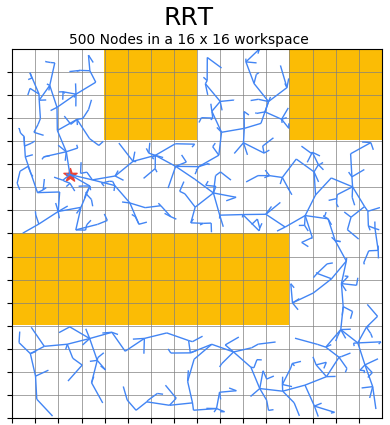
\includegraphics[width=0.45\linewidth]{chapters/chapter2/img/rrt_2d_1.png} & 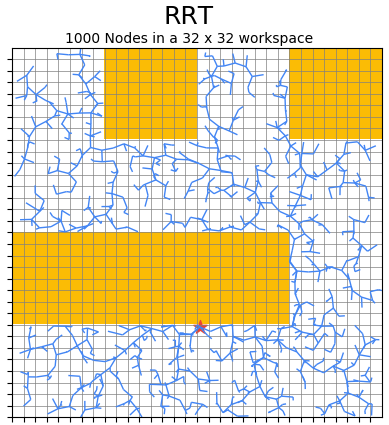
\includegraphics[width=0.45\linewidth]{chapters/chapter2/img/rrt_2d_2.png} \\
    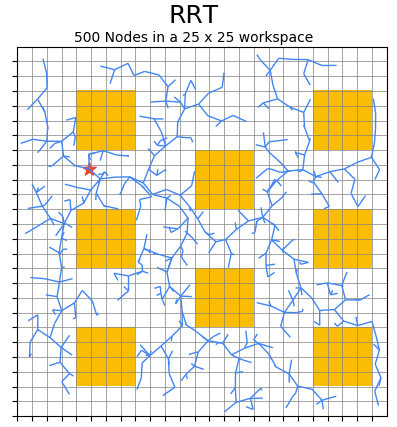
\includegraphics[width=0.45\linewidth]{chapters/chapter2/img/rrt_2d_3.png} & 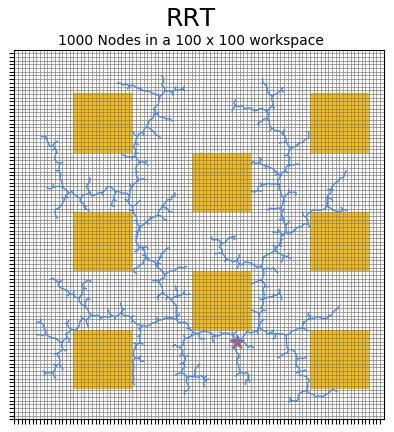
\includegraphics[width=0.45\linewidth]{chapters/chapter2/img/rrt_2d_4.png}
    \end{tabular}
    \caption{2D RRT Implementation shown by \ac{GUI}}
    \label{figure:2DrrtGui}
\end{center}
\end{figure}

    \subsubsection{Implementation in 3D}
    \todo[inline]{Describe implementation in 3D}
    % @Author: AnthonyKenny98
% @Date:   2020-02-23 14:14:12
% @Last Modified by:   AnthonyKenny98
% @Last Modified time: 2020-03-01 13:51:49


\begin{figure}[H]
\begin{center}
    \begin{tabular}{c  c}
    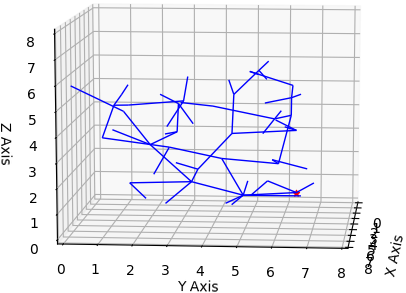
\includegraphics[width=0.45\linewidth]{chapters/chapter2/img/rrt_3d_1.png} & 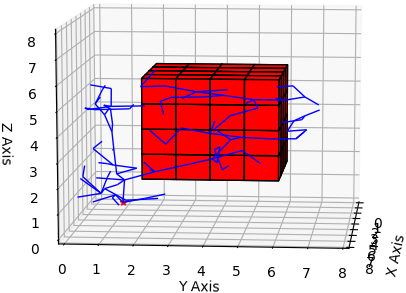
\includegraphics[width=0.45\linewidth]{chapters/chapter2/img/rrt_3d_2.png} \\
    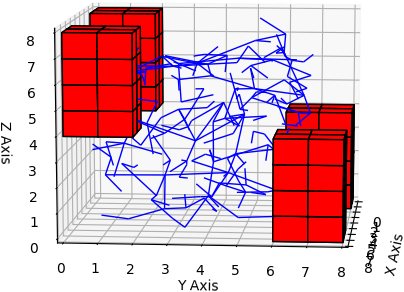
\includegraphics[width=0.45\linewidth]{chapters/chapter2/img/rrt_3d_3.png} & 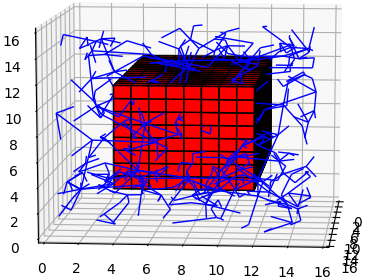
\includegraphics[width=0.45\linewidth]{chapters/chapter2/img/rrt_3d_4.png}
    \end{tabular}
    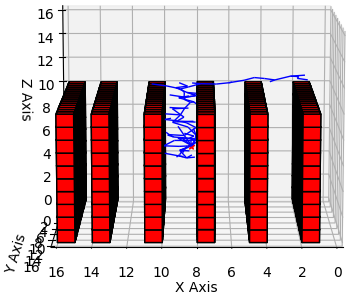
\includegraphics[width=0.45\linewidth]{chapters/chapter2/img/rrt_3d_5.png}
    \caption{3D RRT Implementation shown by \ac{GUI}}
    \label{figure:3DrrtGui}
\end{center}
\end{figure}


\newpage
\section{Analysis of RRT}
\label{section:rrt_analysis}
    % @Author: AnthonyKenny98
% @Date:   2020-02-28 15:02:19
% @Last Modified by:   AnthonyKenny98
% @Last Modified time: 2020-02-28 23:28:59

\todo[inline]{Brief introduction outlining purpose of performance analysis}

\subsection{Methodology}
    To restate, the aim of this thesis is to design a computer processor with reduced execution time of motion planning algorithms, such as \ac{RRT}. As such, it is important to understand the elements of the algorithm that have the highest percentage of CPU execution time. To determine this, it was necessary to implement my own, naive but typical, \ac{RRT} in C. This program could then be compiled and analysed using a software performance profiling tool. With this, I could design experiments to determine the critical RRT functions (those occupying a majority of CPU time) and see how this varies given different parameters.
    \todo[inline]{Outline of method of analysis. Something better than the above}

    \subsubsection{VTune Profiler}
    \label{subsubsection:vtune}
        VTune Profiler performance profiler is an application for software performance analysis. It provides functionality to examine hot-spots for CPU execution time through a top down analysis, shown below in Figure \ref{figure:VTuneTopDown}. As can be seen from the figure, the top down analysis tool shows the percentage of CPU time taken up by each function. I used this tool to profile the algorithm's performance as I changed certain parameters.
        \todo[inline]{Rewrite the above}
        % @Author: AnthonyKenny98
% @Date:   2020-02-23 14:33:19
% @Last Modified by:   AnthonyKenny98
% @Last Modified time: 2020-02-23 14:36:06

\begin{figure}[H]
\begin{center}
    \missingfigure[figwidth=\linewidth]{Screenshot of VTune Top Down Analysis (Maybe)}
    \caption{VTune Amplifier TopDown Analysis Example}
    \label{figure:VTuneTopDown}
\end{center}
\end{figure}

    \subsubsection{Internal Timing}
        The limitation of VTune Profiler is that it can only profile software running on Intel processors, which implement the x86-64 \ac{ISA}. As such, when the time comes to analyse performance of the software running on a RISC-V processor, another method will be required. A simple and effective way of measuring execution performance is to insert timing functionality into the software itself. 

    \subsubsection{Comparison}

\subsection{Results}
\label{section:rrt_analysis_results}